\subsection{The Abstract Syntax Tree}\label{subsec:ast}

The \emph{BookStore} concept
\footnote{For brevity,
only displaying the partial tree of the CML model defined in figure \ref{fig:store} (just for the \emph{BookStore} concept), 
but a similar tree is generated by the compiler for all other concepts.}
specified in the model of figure \ref{fig:store},
when parsed and instantiated by the CML compiler,
generates the following abstract syntax tree (or AST for short):

\begin{figure}
\centering
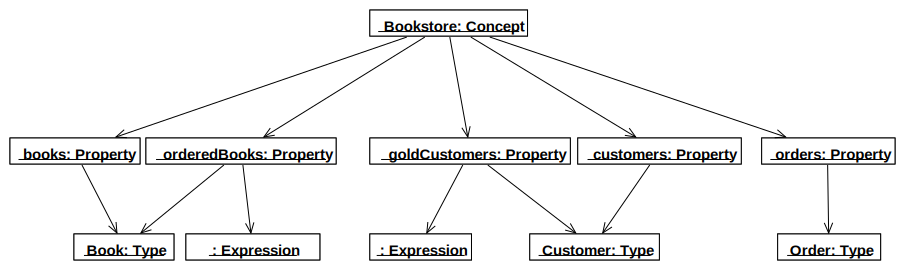
\includegraphics[width=\textwidth]{language/figure-ast}
\caption{The abstract syntax tree generated by the CML compiler after parsing the \emph{BookStore} concept.}
\label{fig:ast}
\end{figure}

The resultant AST in figure \ref{fig:ast} is the CML compiler's internal representation of the \emph{BookStore} concept,
as specified by the model in the CML source listed in figure \ref{fig:store}. 
Using EMOF's terminology \cite{mof},
each node in figure \ref{fig:ast} represents an instance of a class from the CML metamodel.
The root-level node is an instance of the \emph{Concept} class. 
Its subnodes are instances of the \emph{Property} class,
which in turn have (as subnodes) instances of the \emph{Type} and \emph{Expression} classes.

Once generated internally by the CML compiler,
the AST in figure \ref{fig:ast} will be used as the input for the extensible templates during the code generation phase,
shown in section \ref{sec:compiler}.

In order for the CML compiler to successfully generate the AST,
it is necessary to define the CML metamodel,
which is presented in subsection \ref{subsec:metamodel}.
Before, subsection \ref{subsec:mapping} explores the mapping of conceptual models defined with CML to other modeling notations.

